\documentclass[10pt,twocolumn]{article}
\usepackage[margin=0.75in]{geometry}
\usepackage[T1]{fontenc}
\usepackage{lmodern}
\usepackage{graphicx}
\usepackage{booktabs}
\usepackage{amsmath}
\usepackage[numbers,sort&compress]{natbib}
\usepackage[hidelinks]{hyperref}
\usepackage{xcolor}
\usepackage{enumitem}
\setlist{nosep,leftmargin=*}
\graphicspath{{./}}
% Visible marker for anything still to fill in. Remove every one before submission.
\newcommand{\todo}[1]{\textcolor{red}{[TODO: #1]}}

\title{Held-out Accuracy Is Not New-Collection Accuracy:\
A Cross-Collection Benchmark of Poultry Dropping Classifiers\
and a Process-Isolated Pen-Camera Pipeline on a QNX Raspberry Pi 5}
\author{Deekshith Reddy Bhoomireddy \and Rishit Rai \and Lance Streuber}
\date{}

\begin{document}
\maketitle

\begin{abstract}
Deep networks classify photographs of poultry droppings into healthy, coccidiosis, salmonella and Newcastle disease
with reported accuracies of 97.8 to 99.3\%, but these numbers come from random splits of a single collection. We
retrained the classifiers earlier work used (MobileNetV2 and EfficientNet-B0) and our YOLO11n detector on the same
split of the public Tanzanian farm photographs. We then tested all of them on the same 679 held-out farm photographs
and on 1,255 photographs from a separate collection, taken on farms and labelled from PCR tests. Every model scores
98.5 to 99.6\% on the farm test and 75 to 78\% on the PCR-labelled photographs when it always gives an answer, a drop
of 21 to 25 points, and the detector does not differ significantly from either classifier. The farm collection may
explain part of this, because its salmonella and Newcastle photographs come from experimentally inoculated birds. An
audit found 49 farm test photographs (7.2\%) that are exact copies of training photographs, and 19 pairs of identical
PCR files filed under two classes, but neither changes accuracy by more than about one point. The detector's box
score ranks photographs well but is not a calibrated probability. We also graded every PCR-labelled photograph for
appearance with three AI raters (Krippendorff's alpha 0.76). Salmonella droppings look almost healthy, yet the
models still name them correctly, while normal looking coccidiosis is mostly missed. Because a fixed pen camera sees
a dropping as a small object, we fine-tuned the detector on public barn video with real droppings pasted onto the
litter, split by camera. On unseen cameras, recall rises from 0.29 to 0.80 and precision from 0.11 to 0.93, at a cost
of 0.02 mAP50 on close-ups. A pipeline built around the close-up detector runs on a Raspberry Pi 5 under the QNX
microkernel. Each stage is a separate process, and a stage killed with \texttt{SIGKILL} was relaunched within 20 to
33\,ms of the supervisor noticing the exit while the others kept running. We release the code, the per-photograph
predictions and every figure with its data.
\end{abstract}

\section{Introduction}
\label{sec:intro}

Coccidiosis alone was estimated to cost the global chicken industry about \pounds10.4 billion at 2016
prices~\cite{blake2020}. Coccidiosis, salmonellosis and Newcastle disease change the colour and consistency of
droppings, and farmers already look at droppings to judge flock health. This has made dropping photographs a popular
target for deep learning. On the public Tanzanian collection of Machuve et al.~\cite{machuve2022,machuve2021farm},
convolutional classifiers reach 98 to 99\% accuracy~\cite{machuve2022,dhungana2025,degu2023,reyad2024,huda2024}, and
several groups have proposed phone, web or edge systems around them~\cite{degu2023,sakib2026,dhungana2025}.

These accuracies come from random splits of a single collection. A random split by photograph places pictures from
the same farm visit, and sometimes the same picture, on both sides of the split~\cite{barz2020,kapoor2023}. The
original authors wrote that they did not expect their model to be affected by distribution shift~\cite{machuve2022}.
This has not been tested for the four-class task. The same group released a second collection whose labels were
confirmed by PCR~\cite{machuve2021pcr}, which offers a direct test. A second gap is the camera. Published systems
classify close-up photographs taken by a person. A camera fixed above a pen sees each dropping at 8 to 30 pixels,
among birds, feeders and litter, and nobody is there to restart the device when software fails.

We address both gaps with one detector and one honest protocol. Our contributions are as follows.

\begin{enumerate}
\item A benchmark of the classifiers earlier work used (MobileNetV2, EfficientNet-B0) and a ResNet-50 reference,
  retrained on the same split as our YOLO11n detector and tested on the same 679 farm photographs and on 1,255
  lab-confirmed photographs that no model saw. On the farm test our detector calls 97.9\% of photographs correctly,
  in line with published numbers. On the lab-confirmed photographs it calls 67.1\% correctly
  \todo{baseline numbers}. To our knowledge this is the first such test for the four-class task.
\item An audit of the split. We find that 49 of the 679 test photographs (7.2\%) are exact copies of training
  photographs, and we show that removing them changes the farm accuracy by only 0.1 points. We also show that the
  detector's box score is not a calibrated probability.
\item A pen-scale fine-tune trained with real droppings pasted onto barn video frames, split by camera. On cameras it
  never saw, recall rises from 0.29 to 0.80 and precision from 0.11 to 0.93, at a cost of 0.02 mAP50 on close-ups.
\item A complete pipeline running on a Raspberry Pi 5 under the QNX microkernel, with every model timed on the device.
  Each stage is an isolated process. When we kill any stage, it is restarted in 20 to 33\,ms while the others keep
  running. To our knowledge no peer-reviewed work has run poultry health vision on a microkernel real-time operating
  system.
\end{enumerate}

We release the code, the per-photograph predictions, the duplicate hashes and every figure with the table behind it.

\section{Related work}
\label{sec:related}

\paragraph{Classifying poultry droppings.} Machuve et al.\ collected the Tanzanian photographs we use and compared
five convolutional networks~\cite{machuve2022}. With fine-tuning, MobileNetV2 reached 98.02\% and Xception 98.24\% on
a farm-labelled test set, and the authors recommended MobileNetV2 for deployment. Later work on what appear to be the same
photographs, often through a 224-pixel Kaggle copy, reports similar numbers. Degu and Simegn combined a YOLOv3 detector with a
ResNet-50 classifier for a phone application and report 98.7\%~\cite{degu2023}. Reyad et al.\ report 99.25\% with a
majority-vote ensemble~\cite{reyad2024}, and Huda et al.\ 97.78\% with a hybrid of EfficientNetV2-B0 and
DenseNet-121~\cite{huda2024}. The closest pipeline to ours is that of Dhungana et al., a YOLO11n detector followed by
an EfficientNet-B0 classifier, with a detector mAP50 of 0.881 and a classifier accuracy of 99.12\%~\cite{dhungana2025}.
Sakib et al.\ capture photographs with an ESP32-CAM and classify them with EfficientNet-B0 on a server, reporting
99.19\% on a public test set and 95.62\% on a separate local-farm set~\cite{sakib2026}. Other groups built their own
data. Aworinde et al.\ released 14,618 cleaned Nigerian smartphone photographs at $100\times100$
pixels~\cite{aworinde2023}, and Nakrosis et al.\ classified 487 Lithuanian photographs of droppings on litter into six
appearance classes, with 91.78\% accuracy~\cite{nakrosis2023}. Wang et al.\ detected droppings on a conveyor belt
below caged broilers~\cite{wang2019}. Li surveys poultry datasets~\cite{li2025survey}.

\paragraph{Testing beyond one collection.} Bodempudi et al.\ are the closest to our evaluation. They classified
droppings as \emph{Salmonella} PCR positive or negative across United States and African images and report up to
85\% across regions~\cite{bodempudi2026}. Their task is binary and their test set is a different region. We test all
four classes, on a collection from the same group whose labels were confirmed in the laboratory, which separates the
effect of label source and collection from the effect of region. More broadly, leakage between training and test data
has inflated results across many fields~\cite{kapoor2023}, near-duplicate images between the splits of standard
benchmarks have been documented~\cite{barz2020}, and networks often learn shortcuts such as framing or background that
stand in for the class~\cite{geirhos2020}. We use the calibration and selective prediction tools of Guo et
al.~\cite{guo2017} and Geifman and El-Yaniv~\cite{geifman2017}.

\paragraph{Edge deployment and operating systems.} Livestock vision on small devices usually means shrinking the
model, for example by up to 270 times for microcontrollers~\cite{zhang2026tinyml}. Published dropping systems run on a
phone, a server or a laptop~\cite{degu2023,sakib2026,dhungana2025}. None that we found addresses what happens when part
of the software fails on an unattended device. Microkernels move drivers and services into isolated processes, so a
fault stays in one process~\cite{klein2009sel4,qnx8sysarch}. We measure recovery directly.

\section{Methods}
\label{sec:methods}

\subsection{Data}
\label{sec:data}

\paragraph{Farm photographs.} We used the poultry faecal image collection of Machuve et al.\ released on Zenodo
(record 4628934, CC BY 4.0)~\cite{machuve2022,machuve2021farm}. It contains 6,812 full-resolution smartphone
photographs taken in Arusha and Kilimanjaro, Tanzania, with official bounding boxes in YOLO format for four classes:
healthy, coccidiosis, salmonella and Newcastle disease. According to the record, the healthy and coccidiosis
photographs were taken on poultry farms, the salmonella photographs from experimentally inoculated birds one week
after inoculation, and the Newcastle photographs from inoculated birds within three days. Each class therefore comes
with its own setting. We downloaded the archives through the Zenodo API and checked each against the MD5 checksum
the publisher lists. Following the dataset, we refer to the disease classes as \emph{coccidiosis-like},
\emph{salmonella-like} and \emph{Newcastle-like}, because no photograph in this collection carries a laboratory
diagnosis of its own dropping.

\paragraph{Lab-confirmed photographs.} The same group released a second, separate collection of 1,255 photographs
from layer, cross-bred and indigenous chickens on farms in the same two regions, each coded to a faecal sample that
the dataset authors tested by polymerase chain reaction (PCR) (Zenodo record 5801834)~\cite{machuve2021pcr}. We call
them PCR-labelled or lab-confirmed photographs. They contain 373 coccidiosis, 347 healthy, 349 salmonella and 186
Newcastle disease photographs. No model in this study was trained, tuned or selected on any of them. We use them only
as an external test set. The release contains 35 pairs of byte-identical files, so it holds 1,220 distinct images.
In 19 of these pairs the two files sit in different classes (16 coccidiosis and healthy, 3 healthy and salmonella),
so at least 19 labels or file placements are wrong. We report results on all 1,255 files, as released, and give the
effect of removing the 38 conflicting files in Section~\ref{sec:res-bench}.

\paragraph{Barn video.} To teach the detector the size droppings have in a fixed pen camera, we took background
frames from two public video collections of broiler houses: the PIO videos (Zenodo record 16686320, CC BY
4.0)~\cite{boniche2025piodata,boniche2026pio} and the NESTLER poultry videos (Zenodo record 15063494, CC BY 4.0)~\cite{nestler2025}. No dropping in these
videos is labelled, and we did not label any.

\subsection{Split}
\label{sec:split}

The 6,809 farm photographs that have labels (three label files are empty) were split 80/10/10 by photograph within
each class, using a fixed seed on the sorted file names, giving 5,451 training, 679 validation and 679 test
photographs. This is the kind of random split earlier work
on this collection reports. The detector and every baseline in Section~\ref{sec:bench} use exactly this split. To
measure leakage, we reduced every photograph to a 256-bit difference hash~\cite{krawetz2013} and recorded, for
each test photograph, the Hamming distance to the closest training photograph.

\subsection{Detector}
\label{sec:detector}

Our detector is YOLO11n~\cite{jocher2024yolo11} with four classes, fine-tuned from COCO weights at 640 pixels with early stopping (patience 20, seed 0) on a local laptop GPU. The Newcastle-like class has about a sixth of the
photographs of the others, so its training photographs are repeated three times, after the split and in the training
set only. Training stopped at epoch 69 and the weights of epoch 49, the best on validation, were kept
(\texttt{dropping4-laptop}). We exported it to ONNX at 320, 416 and 640 pixels. To check that the result does not depend on the machine, we repeated the training on the Veri cloud
platform on one NVIDIA A10G GPU, with batch 32 and a 30-minute limit (20 epochs). That run reached a test mAP50
of 0.854 and mAP50-95 of 0.573, against 0.873 and 0.573 for the local run, so the two are close. All results below
use the local run.

To compare the detector with photograph classifiers, we score a whole photograph with it: the photograph is
letterboxed to 640 pixels, every candidate box keeps its class scores, and each class takes its best score in the
photograph. The photograph's call is the class with the highest score, or \emph{no detection} when no box reaches
0.25, the confidence threshold the deployed pipeline uses.

\subsection{Pen-scale fine-tuning}
\label{sec:pen}

We handle pen frames at $1280\times720$ and assume that a dropping spans 8 to 30 pixels along its longest side there.
This is a design assumption for a ceiling camera over a pen, not a measurement, since no droppings in our pen videos
are labelled. In the farm collection, by contrast, the disease-class boxes cover a median of 12 to 22\% of the
photograph. We built a pen-scale training set by copy-paste
augmentation~\cite{ghiasi2021}: real labelled droppings were cut from the farm photographs along their
official boxes, shrunk to pen size, and pasted onto empty litter in barn video frames. A dropping from a training
photograph is only ever pasted into a training tile, and likewise for validation and test, so the farm split carries
over. Background frames were split \emph{by camera}, never by frame. Five PIO videos and the remaining NESTLER cameras
form the training set, one NESTLER camera the validation set, and three NESTLER cameras plus the PIO video used in our
live demonstration the test set. Frames with birds and equipment and no pasted dropping were kept as negatives. The
model \texttt{dropping4-pen} was fine-tuned from \texttt{dropping4-laptop} on these tiles mixed with the original
farm photographs, for up to 40 epochs (patience 10). It stopped at epoch 38.

We state the limitation plainly: the pen test is synthetic. It measures whether the model finds a real dropping of
pen size on litter and cameras it has never seen, not field accuracy on naturally occurring droppings.

\subsection{Baselines}
\label{sec:bench}

Published results on this collection come from different splits, image sizes and protocols, so we retrained the
classifiers earlier work used instead of quoting their numbers. MobileNetV2~\cite{sandler2018} is the model
Machuve et al.\ recommended for deployment~\cite{machuve2022}, EfficientNet-B0~\cite{tan2019} is the
classifier stage of a recent YOLO11 and EfficientNet-B0 pipeline~\cite{dhungana2025}. Each was
initialised from ImageNet weights and trained on the same 5,451 training photographs, resized to $224\times224$
without keeping the aspect ratio (as in the 224-pixel copy of the collection most earlier work used), with AdamW and a
one-cycle learning rate schedule. MobileNetV2 was trained for 20 epochs and EfficientNet-B0 for 8, both with one seed,
because of the compute time available to us. Augmentation
was random crops, horizontal and vertical flips, and small brightness and contrast changes. We did not change hue,
because colour is the main visual sign of disease. The epoch with the best validation accuracy was kept. Both passed 98\% validation accuracy within four epochs, so the shorter EfficientNet-B0 run is unlikely to change
the comparison, but one seed cannot measure run-to-run variation.

\subsection{Evaluation}
\label{sec:eval}

All models are scored on the same 679 farm test photographs and the same 1,255 lab-confirmed photographs. We report
accuracy, per-class recall and macro-F1. Proportions carry 95\% Wilson score intervals~\cite{wilson1927}, which
behave well near 0 and 1. For the detector we also report a risk-coverage curve~\cite{geifman2017}, the
accuracy of the answers when the model only answers above a confidence threshold, and a reliability diagram with the
expected calibration error over ten equal-width bins~\cite{guo2017}.

\subsection{Appearance grades for the lab-confirmed photographs}
\label{sec:grades}

PCR says whether a pathogen is in the sample, not how the dropping looks. To ask whether the models fail on
droppings that look normal, we graded every one of the 1,255 lab-confirmed photographs for appearance. A written
rubric scores six visual variables 0, 1 or 2, or leaves them empty when the photograph does not show them: form,
the white urate cap, colour, blood, mucus or foam, and undigested feed. These are the signs used in clinical checks
of droppings. The grade is computed, never chosen, as $\max(1, 10 - p)$ where $p$ is the sum of the six scores with
blood counted twice, so every lost point has a named reason. Grades 9 and 10 mean the dropping looks normal.

The raters were three AI vision models, not people: Claude Opus, Claude Sonnet and Claude Haiku, each run with
the same written instructions and no shared context. Each photograph got a random identifier and was re-encoded
at 768 pixels with no metadata, and the key linking identifiers to file names and PCR classes stayed outside the
raters' folder until grading ended. Each rater saw the photographs in its own random order. 126 photographs (10\%)
were shown a second time under a new identifier to measure each rater's agreement with itself. The released
sub-score for a photograph is the median of the raters who could judge it, needing at least two, and its grade is
recomputed from those medians. We report Krippendorff's alpha for ordinal data across the three
raters~\cite{hayes2007} and quadratic weighted kappa for each pair and for each rater against itself~\cite{cohen1968}.

\subsection{Deployment on QNX}
\label{sec:qnx}

The deployed system runs on a Raspberry Pi 5 with a Camera Module 3 under QNX 8.0, a microkernel real-time operating
system~\cite{qnx8sysarch}. The pipeline is split into separate processes (sections), each with its own memory and a
fixed real-time priority: camera capture in C, a still-spot finder that flags new objects that appeared and stayed
still, the detector, an explanation step, and links to the dashboard and a wrist-worn display. Full frames stay in a
shared-memory ring of four slots, and sections exchange only small messages through QNX native message passing. A
supervisor restarts any section that exits. On the Pi the detector is the close-up model, run on a full-resolution
patch around each candidate from the spot finder, not the pen model. At pen scale the close-up model can score white
birds as salmonella, so the explanation step dismisses a candidate unless its box lies on the spot, has the size of a
dropping, is not white, is not lighter than the floor around it, and scores at least 0.6. Inference uses ONNX Runtime~\cite{onnxruntime} 1.24.4 from the QNX
open-source package repository, called from a small C bridge because the repository's Python binding does not load on
QNX (Section~\ref{sec:discussion}). We report the detector's inference time on the Pi with four threads, without image
decoding or post-processing.

Alerts reach people in two ways. A wrist-worn display polls the dashboard and shows each pen's state. A separate
messaging service sends pen alerts to the farmer over iMessage through the Photon platform and answers follow-up
questions in plain language with a large language model (DeepSeek). Each alert states what the camera recorded, the
model's closest match with its score, and that it is not a laboratory test. The service never tells the farmer to
treat or cull birds. It contacts a veterinarian only after the farmer clearly agrees, and that decision is made by
tested rules in the application code, not by the language model. We describe this service for completeness and do not
evaluate it here. Figures~\ref{fig:hardware} and~\ref{fig:interfaces} show the hardware and the three interfaces.

\begin{figure*}[t]
\centering
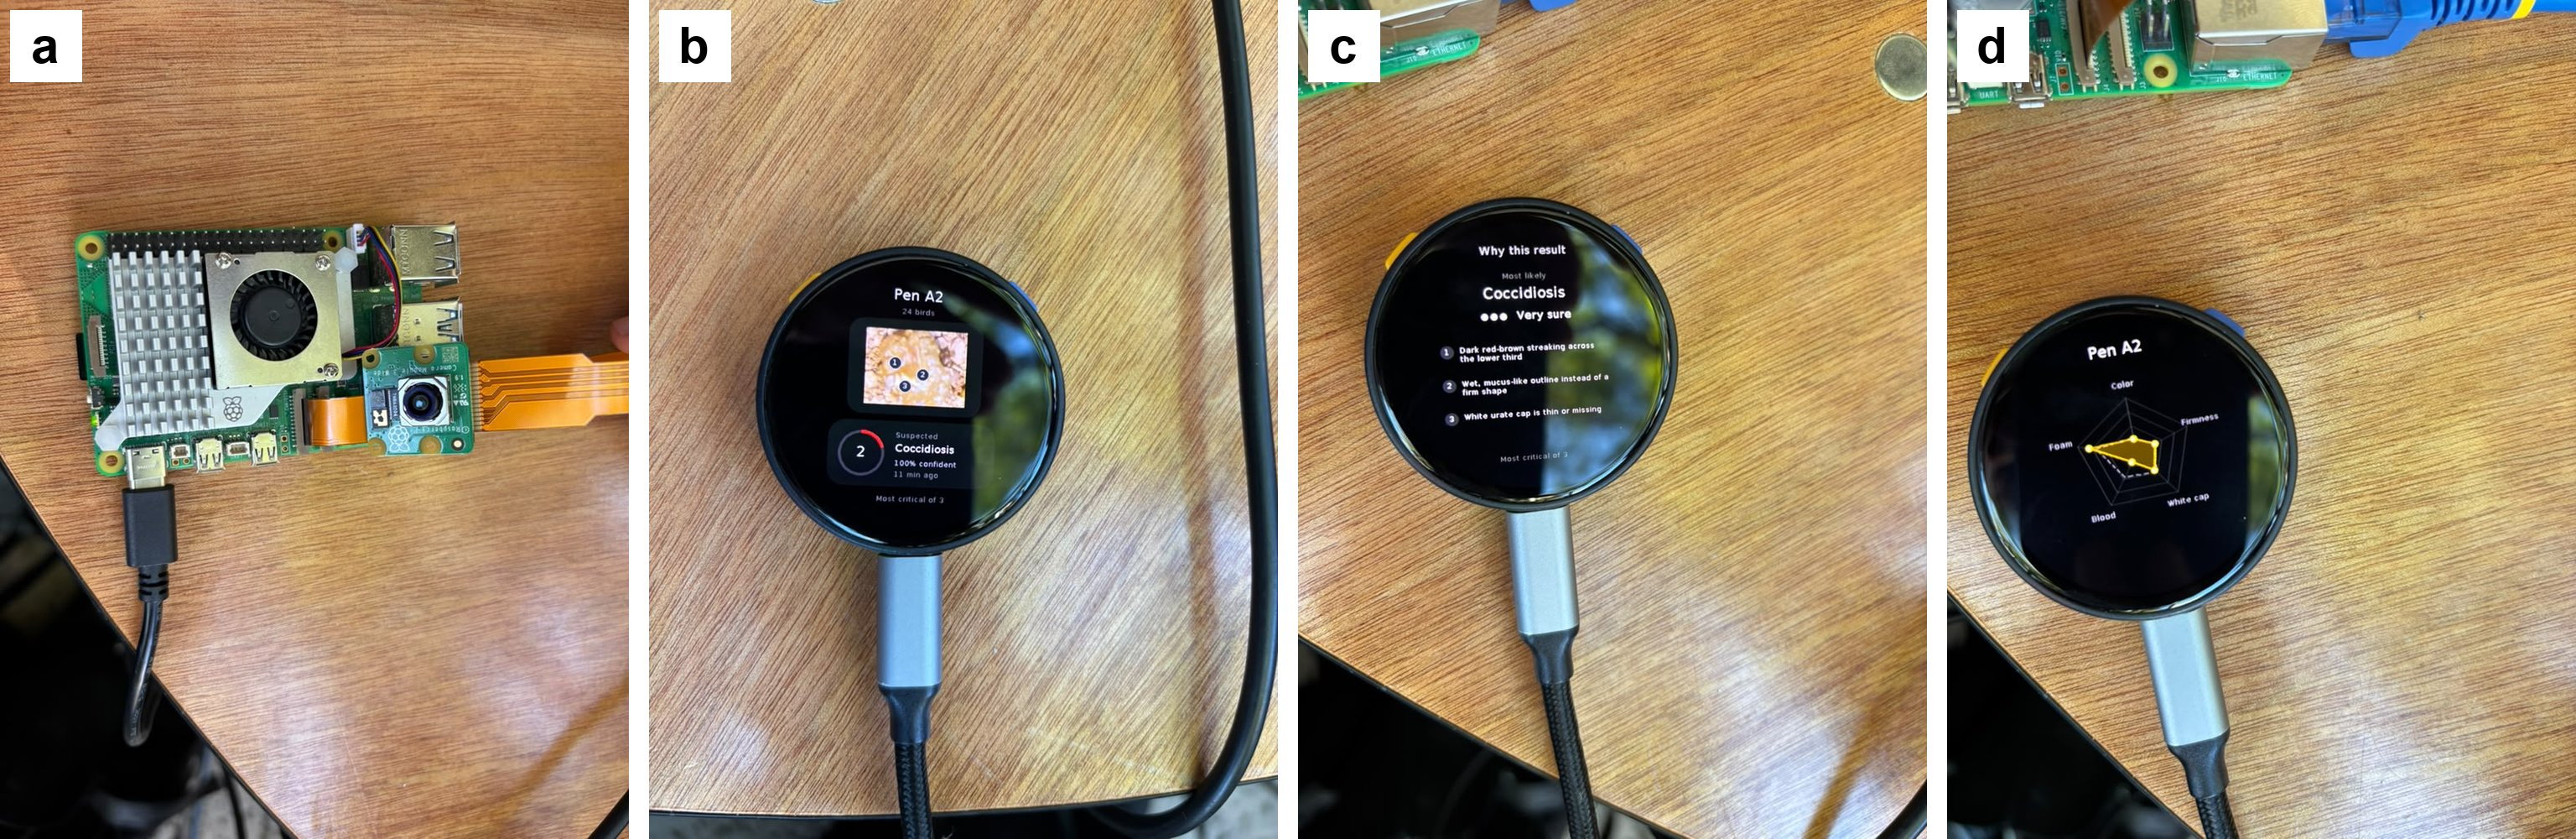
\includegraphics[width=\textwidth]{figures/system_hardware.jpg}
\caption{The deployed hardware. (a) Raspberry Pi 5 running QNX 8.0 with a Camera Module 3 on its ribbon cable and an
active cooler. (b to d) The wrist-worn display (M5Stack StopWatch) on its charging cable, showing a pen's newest
specimen with its photograph and numbered evidence markers (b), the evidence in words (c), and the pen's five
appearance checks against the barn average (d). The display is shown with the dashboard's demonstration data, not a
field reading.}
\label{fig:hardware}
\end{figure*}

\begin{figure*}[t]
\centering
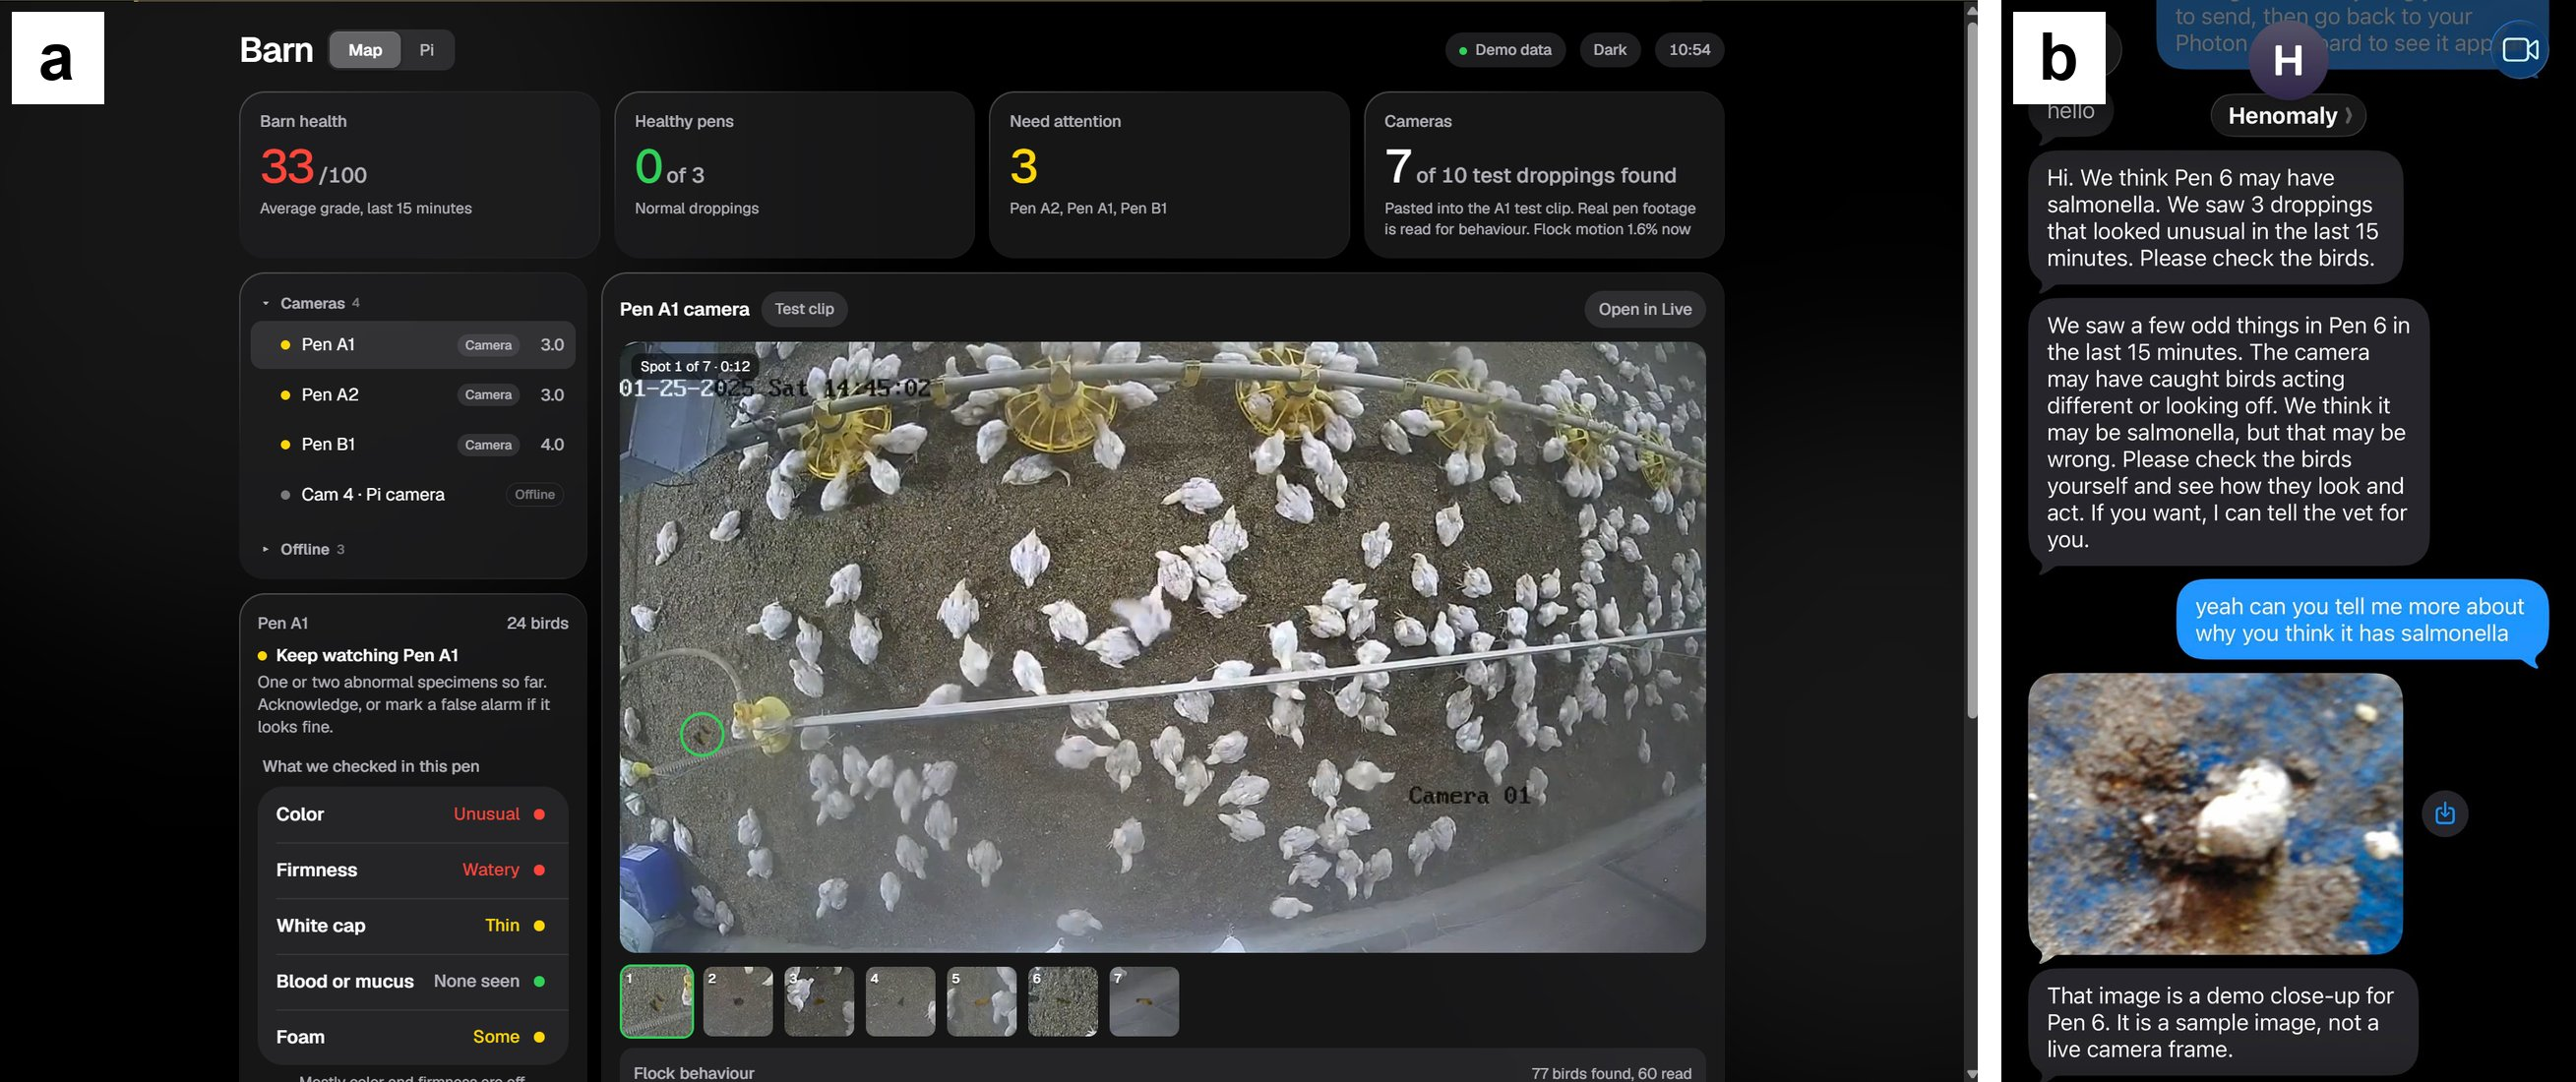
\includegraphics[width=\textwidth]{figures/system_interfaces.jpg}
\caption{The two other interfaces. (a) The dashboard with the held-out Pen A1 test clip, in which test droppings were
pasted at known times. A green ring marks a flagged spot and the strip below lists the seven spots found. Pen
readings on the dashboard are demonstration data, as its header states. (b) The farmer messaging service in a test
conversation. The attached photograph is a sample image, as the agent itself says, not a live camera frame.}
\label{fig:interfaces}
\end{figure*}

\section{Results}
\label{sec:results}

\subsection{All models drop on lab-confirmed photographs}
\label{sec:res-bench}

Table~\ref{tab:bench} and Figure~\ref{fig:bench} compare every model on the two test sets. On the farm test all of
them are in the range earlier work reports. MobileNetV2 calls 99.6\% of the 679 photographs correctly \todo{mean over
seeds}, and our detector 98.5\% when it always gives its best guess. On the 1,255 lab-confirmed photographs every model
loses more than 20 points. MobileNetV2 falls to 74.6\% and the detector to 76.3\% \todo{final means and ranges}. The
Wilson intervals of the two test sets do not overlap for any model, so the drop is not sampling noise.

Our detector does not classify better than the classifiers earlier work used. The differences between models on the
lab-confirmed photographs are small next to the drop that every model shows. Under this protocol the published
accuracies of 98 to 99\% describe photographs like the training photographs, and the choice of architecture matters
less than the choice of test set.

\begin{table}[t]
\centering
\caption{Accuracy and macro-F1 on the held-out farm test (679 photographs) and the lab-confirmed photographs (1,255),
for models trained on the same 5,451 photographs. Classifiers: mean over three seeds, range in brackets.
Detector: one run, scored with its best class in each photograph (always answers) and with the deployed 0.25
confidence threshold (below it the photograph counts as wrong).}
\label{tab:bench}
\small
\begin{tabular}{lcccc}
\toprule
& \multicolumn{2}{c}{Farm test} & \multicolumn{2}{c}{Lab-confirmed} \\
Model & Accuracy & Macro-F1 & Accuracy & Macro-F1 \\
\midrule
MobileNetV2~\cite{machuve2022} & \todo{} & \todo{} & \todo{} & \todo{} \\
EfficientNet-B0~\cite{dhungana2025} & \todo{} & \todo{} & \todo{} & \todo{} \\
ResNet-50 & \todo{} & \todo{} & \todo{} & \todo{} \\
YOLO11n (ours), always answers & 98.5 & 98.3 & 76.3 & 75.1 \\
YOLO11n (ours), 0.25 threshold & 97.9 & 97.7 & 67.1 & 70.3 \\
\bottomrule
\end{tabular}
\end{table}

\begin{figure}[t]
\centering
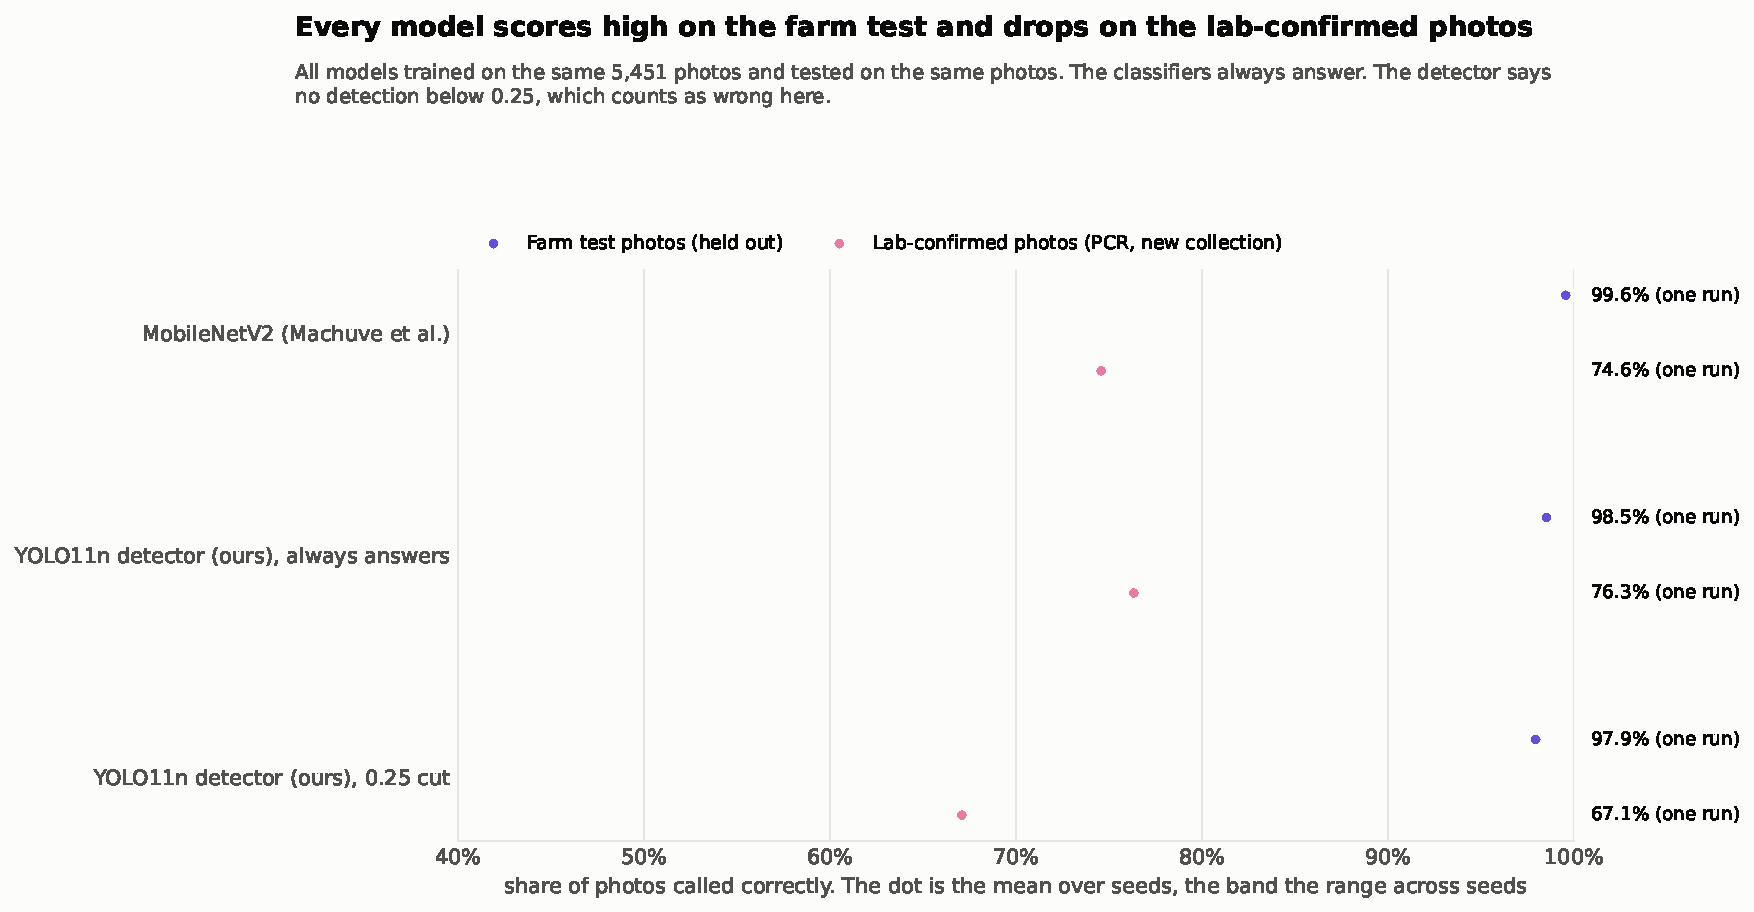
\includegraphics[width=\linewidth]{figures/13_benchmark.pdf}
\caption{Accuracy of each model on the farm test and on the lab-confirmed photographs. Dots are the mean over seeds,
bands the range across seeds. Values are written beside each mark.}
\label{fig:bench}
\end{figure}

\subsection{Where the errors go}
\label{sec:res-errors}

Figure~\ref{fig:confusion} shows the detector's calls on both sets. On the farm test the diagonal holds 95 to 100\% of
every class. On the lab-confirmed photographs most errors are not confusions between diseases. They are photographs
with no detection at all (20\% of healthy and 27\% of Newcastle-like photographs) and photographs called healthy or
salmonella-like by mistake. Newcastle-like recall falls the most, from 94.6\% (35 of 37) to 41.9\% (78 of 186). This
class has 376 photographs in the whole farm collection, against more than 2,000 for each of the others
(Figure~\ref{fig:recall}).

\begin{figure}[t]
\centering
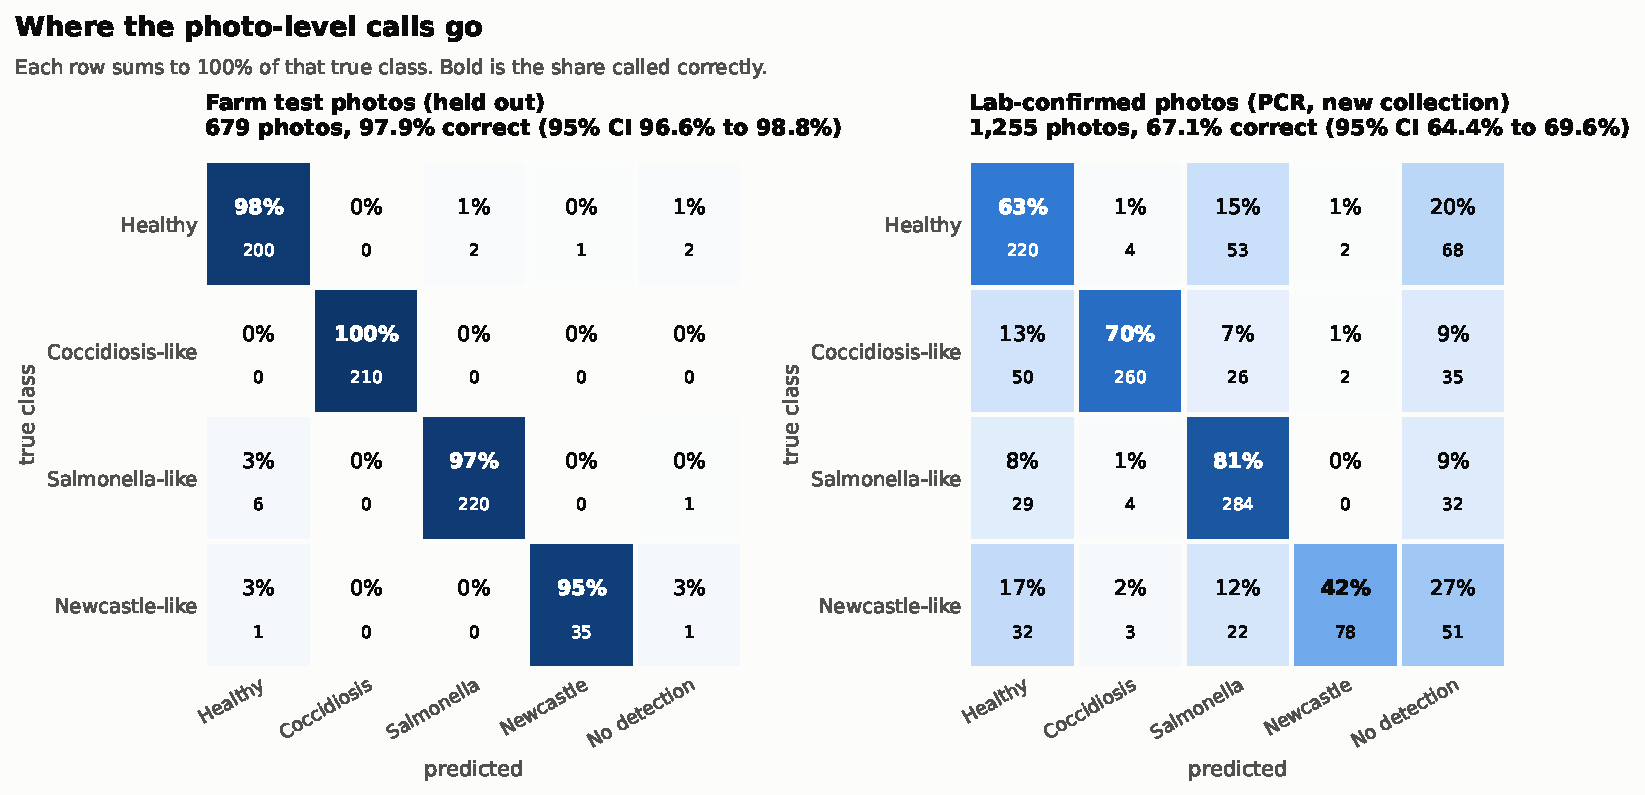
\includegraphics[width=\linewidth]{figures/06_confusion_matrices.pdf}
\caption{Detector calls per true class on the farm test (left) and the lab-confirmed photographs (right). Each row
sums to 100\%. Counts under each share.}
\label{fig:confusion}
\end{figure}

\begin{figure}[t]
\centering
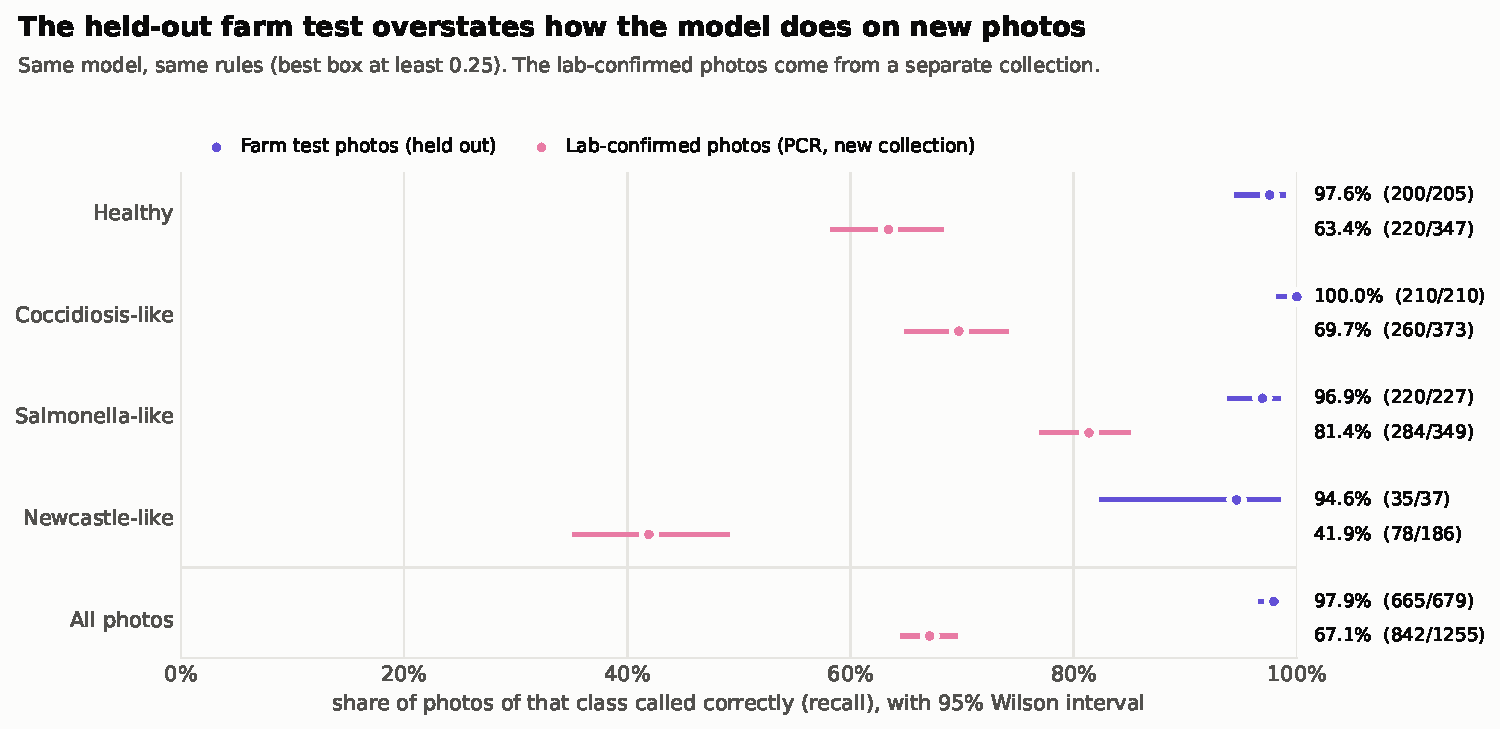
\includegraphics[width=\linewidth]{figures/07_recall_by_class.pdf}
\caption{Per-class recall of the detector with 95\% Wilson intervals, at the deployed 0.25 threshold.}
\label{fig:recall}
\end{figure}

\subsection{Duplicates do not explain the farm score}
\label{sec:res-dup}

Forty-nine of the 679 farm test photographs (7.2\%) have a training photograph with an identical 256-bit difference
hash, and inspection of the closest pairs shows they are the same image saved under two file names
(Figure~\ref{fig:dup}). Every other test photograph differs from its nearest training photograph in at least 40
bits. The detector calls all 49 copies correctly. Without them its farm accuracy is 97.8\% (95\% CI 96.3 to 98.7\%),
against 97.9\% with them. The copies are a flaw in the split, but they are not why the farm test overstates
performance on new photographs.

\begin{figure}[t]
\centering
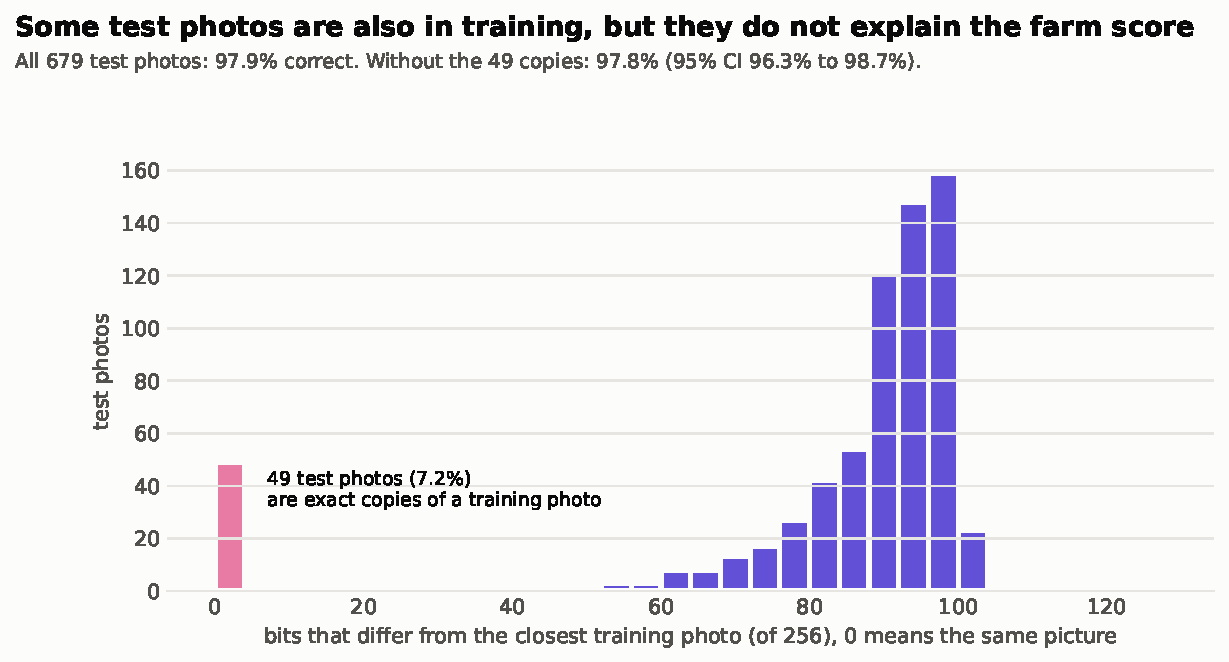
\includegraphics[width=\linewidth]{figures/10_duplicates_across_split.pdf}
\caption{Hamming distance from each farm test photograph to its nearest training photograph (256-bit difference
hash). The bar at zero holds the 49 exact copies.}
\label{fig:dup}
\end{figure}

\subsection{The box score ranks well but is not a probability}
\label{sec:res-cal}

If the detector only answers when its best box clears a threshold, its answers become more reliable
(Figure~\ref{fig:coverage}). On the lab-confirmed photographs, raising the threshold from 0.25 to 0.80 raises the
accuracy of the answers from 78.8\% to 87.4\%, but the detector then answers only 27.8\% of photographs. Its scores
are also under-confident on both sets (Figure~\ref{fig:calibration}). The expected calibration error is 0.177 on the
farm test and 0.172 on the lab-confirmed photographs, and in both cases the photograph is right more often than the
score says. The score should therefore be calibrated, for example by temperature scaling~\cite{guo2017} on the
validation split, before it is shown to a farmer as a percentage.

\begin{figure}[t]
\centering
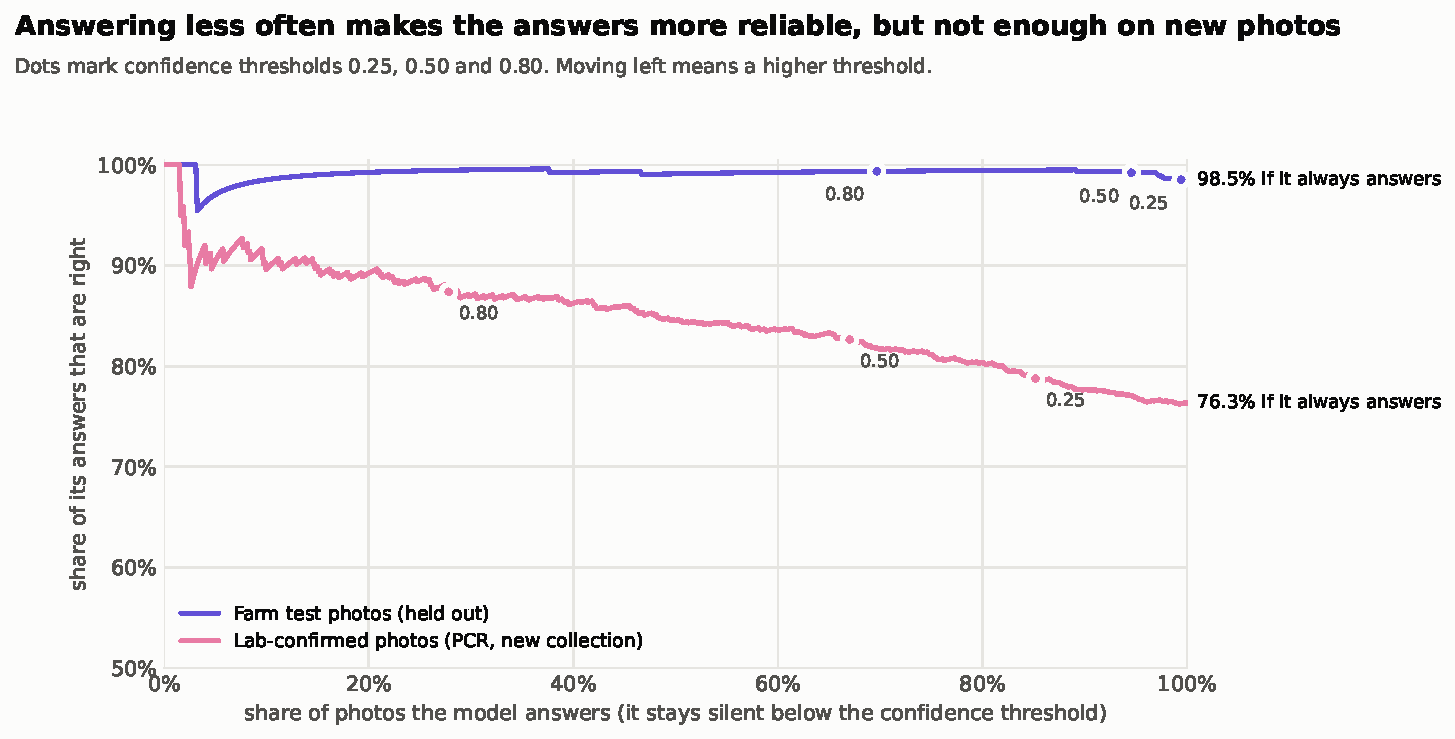
\includegraphics[width=\linewidth]{figures/08_accuracy_vs_coverage.pdf}
\caption{Accuracy of the detector's answers against the share of photographs it answers, as the confidence threshold
rises. Dots mark the thresholds 0.25, 0.50 and 0.80.}
\label{fig:coverage}
\end{figure}

\begin{figure}[t]
\centering
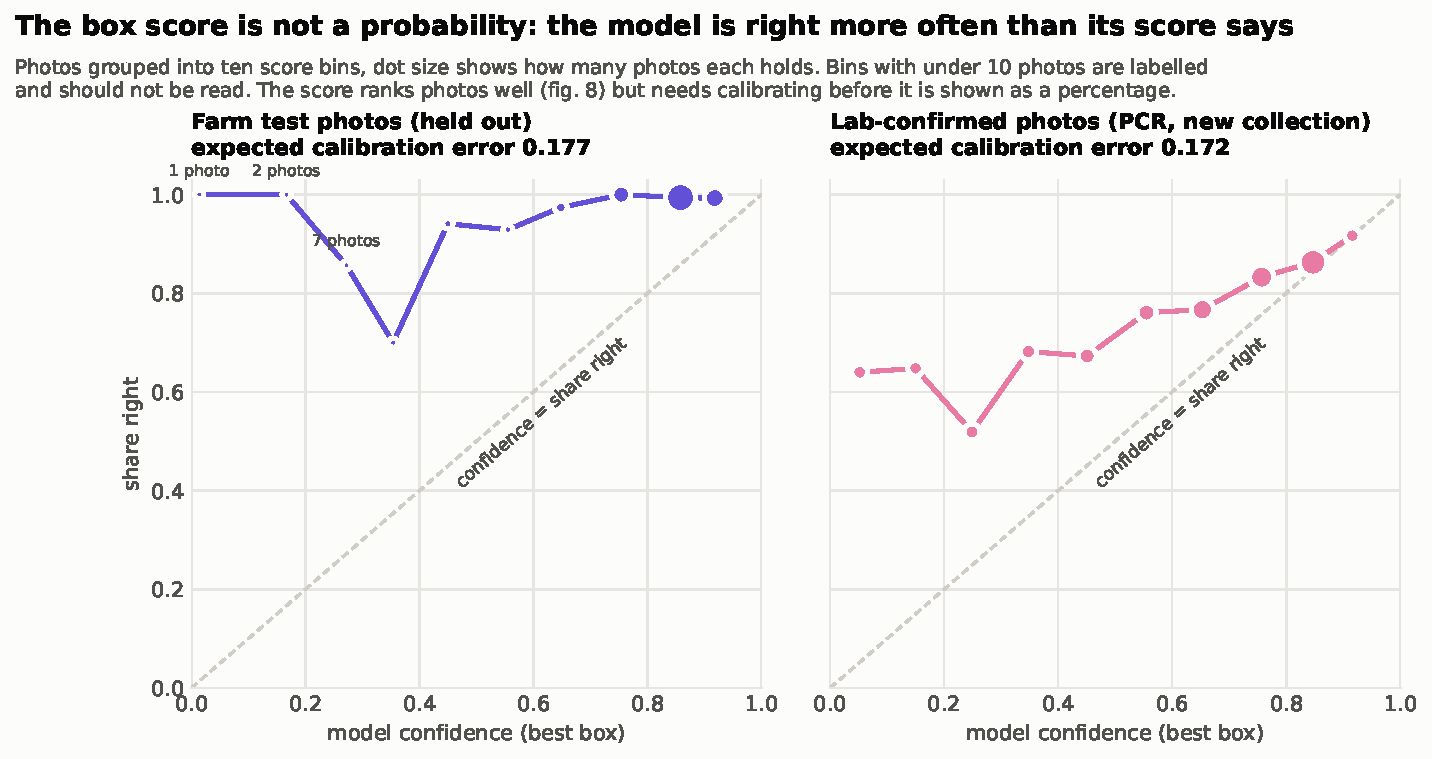
\includegraphics[width=\linewidth]{figures/09_calibration.pdf}
\caption{Reliability diagrams over ten score bins. Dot size shows the number of photographs in a bin. Bins with fewer
than ten photographs are labelled and should not be read.}
\label{fig:calibration}
\end{figure}

\subsection{Pen-scale detection}
\label{sec:res-pen}

The close-up detector does not work at pen scale (Figure~\ref{fig:pen}). On the held-out pen cameras it finds 29\% of
droppings, only 11\% of its boxes are droppings, and it places 3.55 boxes on an average empty pen tile at the 0.25
threshold. After pen-scale fine-tuning, recall is 0.80 and precision 0.93 on cameras the model never saw, and false
boxes on empty tiles fall to 0.05 per tile. The close-up mAP50 changes from 0.873 to 0.853. Class accuracy at pen
size remains weaker than detection (four-class mAP50 0.65). The pen model should therefore find a dropping, and a
full-resolution patch or a close-up photograph should be judged by the close-up model.

\begin{figure}[t]
\centering
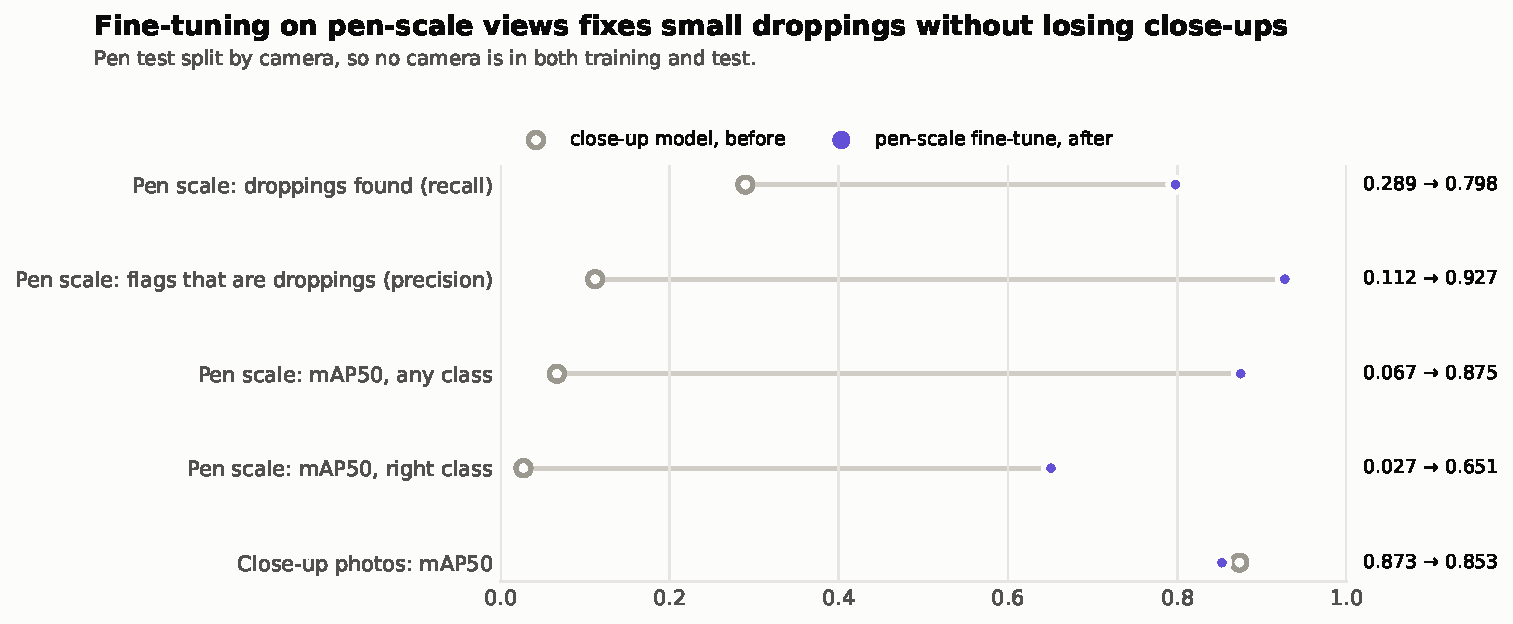
\includegraphics[width=\linewidth]{figures/11_pen_scale_before_after.pdf}
\caption{Pen-scale test on held-out cameras before (close-up model) and after fine-tuning. The pen test uses real
droppings pasted onto real litter.}
\label{fig:pen}
\end{figure}

Whole-photograph classifiers cannot be tested this way. They return one label for an image, and in a pen frame a
dropping covers at most about 0.1\% of the image. Locating the dropping is what makes the pen camera usable, and it is
the main reason to use a detector in this setting rather than a better classifier.

\subsection{The deployed pipeline}
\label{sec:res-qnx}

We also ran the pen model over a three-minute clip from the held-out PIO camera, into which ten test droppings were
pasted at known times. Read at two frames a second with a short persistence rule, it flagged seven, five of them
within two seconds of their appearance, and raised no false flags (Figure~\ref{fig:live}). This run was made on a
laptop, and like the pen test it uses pasted droppings. On the Pi, the deployed pipeline proposes candidates with a
still-spot finder and judges a full-resolution patch of each with the close-up detector. On the Raspberry Pi
5 the detector takes 168\,ms at 320 pixels and 618\,ms at 640 pixels with four threads, and the pen model 608\,ms at
640 pixels \todo{full timing table for all models under the same harness}. Native message passing between two
sections takes 95\,$\mu$s for a 57.6\,KB frame and reply. When we killed any section with \texttt{SIGKILL}, the
supervisor restarted it in 20 to 33\,ms. Killing the spot finder cost the camera one frame and the other sections
none.

\begin{figure}[t]
\centering
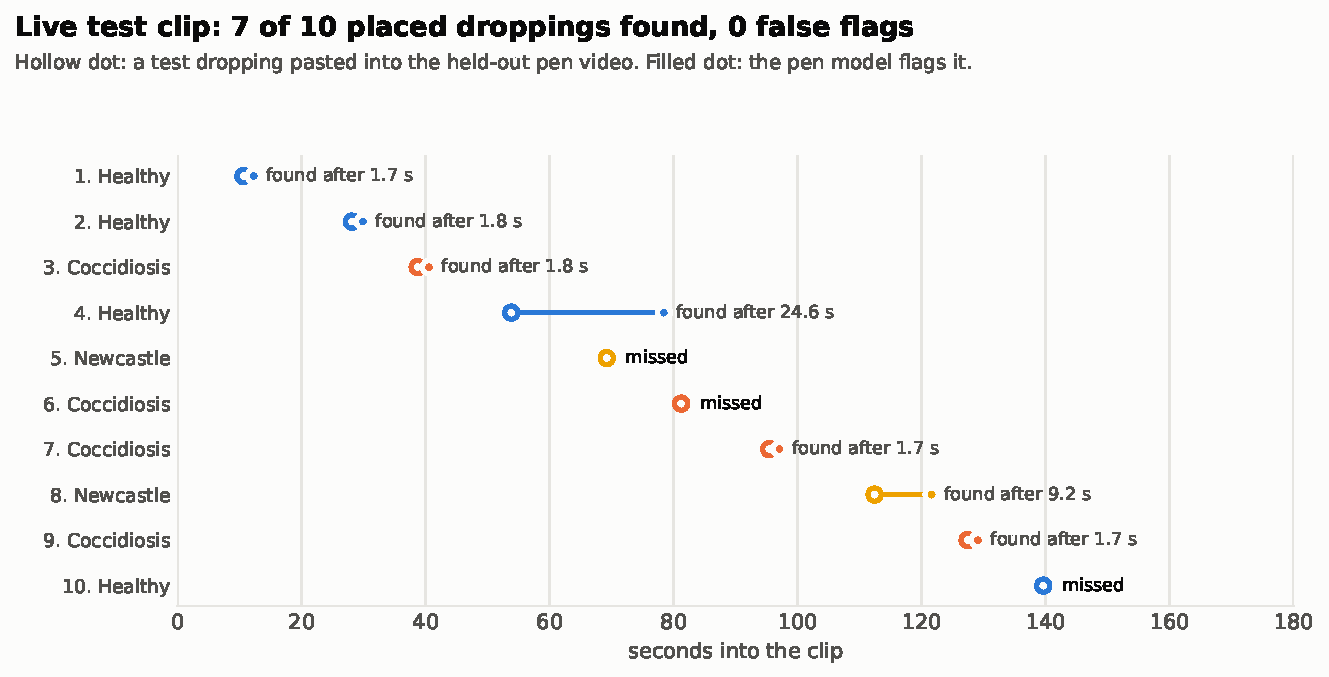
\includegraphics[width=\linewidth]{figures/12_live_clip_answer_key.pdf}
\caption{Test clip with an answer key. Hollow dots mark when each pasted dropping appears in the held-out video,
filled dots when the pen model flagged it.}
\label{fig:live}
\end{figure}

\section{Discussion}
\label{sec:discussion}

\paragraph{What the farm test measures.} Every model we trained, including the two that earlier work recommended,
reaches 98.5 to 99.6\% on the random farm test and loses 21 to 25 points on photographs from a second collection of
the same group. The original authors did not expect distribution shift to matter~\cite{machuve2022}. Our results show
that it matters more than the choice of network. We cannot say from these data which difference between the
collections causes the drop, but the farm collection itself suggests a strong candidate. Its salmonella and
Newcastle photographs come from experimentally inoculated birds and its healthy and coccidiosis photographs from
farms~\cite{machuve2021farm}, while every PCR-labelled photograph comes from a farm. A model can then learn the
setting of each class, such as the surface, the lighting or the birds, along with the dropping, which is the kind of
shortcut described by Geirhos et al.~\cite{geirhos2020}. Healthy droppings in the farm collection also fill a median
of 2.6\% of the photograph, against 12 to 22\% for the other classes, so framing could act as a shortcut too. Three
observations fit this reading without proving it. Exact duplicates are not the cause, because removing them leaves
the farm score unchanged, and neither are the conflicting PCR files, which move every model by about one point. Most
errors are missed detections and calls of healthy or salmonella-like, not swaps between the diseases. And on
normal-looking PCR-labelled photographs the models lean towards salmonella (Section~\ref{sec:grades-results}), the class
whose training photographs came from one inoculation setting. We have not tested these shortcuts directly. Sakib et
al.\ saw a much smaller drop, from 99.19 to 95.62\%, on a local-farm set~\cite{sakib2026}. Their abstract does not say
how that set was labelled or collected, so we cannot tell whether it shares the setting of the training photographs.
Bodempudi et al.\ reached at most 85\% across regions for a binary \emph{Salmonella} task~\cite{bodempudi2026}.
Together these results suggest that published accuracies on this task should be read as within-collection
accuracies.

\paragraph{Why use a detector.} On photographs our detector is not more accurate than a whole-image classifier. Its
value is that it says where the dropping is. That is what makes a fixed pen camera usable, because under our size
assumption a dropping covers at most about 0.1\% of a pen frame, and it is also what lets the explanation step
measure the colour of the dropping itself rather than the litter around it. The pen-scale fine-tune shows that the
detector can learn the size and setting of a pen camera from public video and pasted droppings alone, without a
single labelled pen dropping. It lost 0.02 mAP50 on close-ups in the process. The deployed Pi pipeline does not use
the pen model yet. It finds candidates with a still-spot finder and judges them with the close-up model, whose false
alarms on white birds the explanation step filters out.

\paragraph{Why a microkernel.} A monitor in a barn runs unattended, and a crash in a camera driver or a model runtime
should cost a few frames, not the device. On QNX each stage of our pipeline is an ordinary process, and the
supervisor relaunched any stage we killed within 20 to 33\,ms of noticing the exit while the others kept running. The
same structure is possible on Linux with process supervision. What QNX adds is that the drivers, the file system and
the network stack are also user processes that can fail and restart the same way~\cite{qnx8sysarch}, but our tests
killed only our own stages, not a QNX driver or service. We did not compare fault recovery against Linux on the same
board, so we do not claim QNX recovers faster. Running the model on QNX also needed one fix in the platform's
packages. The Python binding of ONNX Runtime in the QNX open-source repository does not load, because its build
script treats QNX as Windows and looks for the wrong extension module. We worked around it with a 111-line C bridge
to the runtime's C library and have prepared a patch for the package recipe.

\paragraph{Limitations.} All photographs come from one region of Tanzania and one research group. No farm photograph
carries a laboratory diagnosis of its own dropping, two farm classes come from inoculated birds, and the PCR release
contains files filed under two classes, so we treat the classes as screening categories, not diagnoses. The farm
split is random by photograph because the release carries no farm or visit information. The pen test and the test
clip use real droppings pasted onto real barn frames, so they measure whether a pen-sized dropping can be found on
unseen litter, not field accuracy on naturally occurring droppings. The pen size of 8 to 30 pixels is an assumption.
We have no labelled droppings from a real pen camera, and we have not measured the detection accuracy of the deployed
pipeline. The detector and each baseline were trained once, with one seed and one set of hyperparameters that we did
not tune, and EfficientNet-B0 for only 8 epochs. Run-to-run variation is therefore not measured. To explain the drop it
would have to exceed 20 points, far beyond the 0.02 mAP50 gap between our two detector runs on the farm test.
Finally, the edge timings are for inference only and do not include image decoding, post-processing or power draw.
The appearance grades come from three AI models following a rubric, not from veterinarians. Their agreement shows
the grades are consistent, not that they are right, and three models from one vendor may share blind spots. The
rubric is new and has not been validated against expert grading.

\paragraph{Future work.} The most useful next step is labelled droppings from fixed pen cameras on more than one
farm, split by farm. Short of that, the farm collection could be re-split with near-duplicate removal before
splitting, the size shortcut could be tested by cropping every class to the same framing, and the setting shortcut by
testing on salmonella and Newcastle photographs taken on farms. On the device, the next steps are a Linux baseline on
the same Raspberry Pi 5 and fault tests that kill QNX services, not only our own stages. The box score needs
calibration before it is shown to a farmer, and the 0.25 threshold should be chosen from a risk-coverage curve on
validation data rather than fixed.

\section{Conclusion}
\label{sec:conclusion}

Classifiers of poultry droppings that score 98.5 to 99.6\% on a random split of the Tanzanian farm photographs score
75 to 78\% on PCR-labelled photographs from a second collection taken on farms, and this holds for every architecture
we tried, including our detector. We therefore recommend that future work on this task report a second collection
alongside the farm test. A detector cannot fix this drop, but it is what makes a fixed pen camera usable. Fine-tuned
on public barn video with pasted droppings, our YOLO11n detector finds 80\% of pen-sized droppings on unseen cameras
with 93\% precision. A pipeline built around the close-up detector runs on a Raspberry Pi 5 under QNX, where a stage
killed with \texttt{SIGKILL} is relaunched within tens of milliseconds while the rest keeps running.


\section*{Data and code availability}
The farm and lab-confirmed photographs are Zenodo records 4628934 and 5801834, the PIO and NESTLER videos Zenodo
records 16686320 and 15063494, all under CC BY 4.0. Our code, trained weights, per-photograph predictions,
duplicate hashes, appearance grades with every rating, training logs and every figure with the table behind it are at
\url{https://github.com/RishitRai/Holy-Crap}. The figures
are produced by \texttt{data-visualization/evaluation.py}, the baselines by
\texttt{training/benchmark\_classifiers.py}, and the image audit by \texttt{data-visualization/audit\_images.py}.

\section*{Ethics}
This study used only published photographs and videos. No animals were handled and no new animal data were collected.

\section*{Compute}
The detector, the pen-scale fine-tune and the baselines were trained on a local laptop GPU. The pen-scale fine-tune,
the two baselines and every evaluation in this paper ran on an NVIDIA GeForce RTX 4060 Laptop GPU with 8\,GB of memory.
The replicate detector run was trained on the Veri cloud platform on one NVIDIA A10G GPU (job \texttt{abe1b30a56c4}).
All on-device timings were measured on a Raspberry Pi 5 running QNX 8.0.

\section*{Use of AI tools}
The appearance grades in Section~\ref{sec:grades} were produced by three AI models, as described there. AI coding
and writing assistants were used to write analysis code and to draft and edit the text. The authors checked every
number against the released result files and every reference against its source, and take responsibility for the
content.

\section*{Acknowledgements}
We thank Machuve and colleagues for releasing the farm and PCR-confirmed photographs, and the authors of the PIO and
NESTLER datasets for releasing their barn videos, all under open licences. We thank the QNX team for the QNX
Everywhere program and the open-source package repository at \url{https://oss.qnx.com}, whose ONNX Runtime, Python
and numpy builds made on-device inference possible, and Veri for the cloud GPU time used for the replicate training
run. This work was carried out at LA Hacks, in its QNX and Veri tracks. We also thank the developers of Ultralytics
YOLO, PyTorch and ONNX Runtime.

\bibliographystyle{plainnat}
\bibliography{references}

\end{document}
